\documentclass[twoside]{book}

% Packages required by doxygen
\usepackage{fixltx2e}
\usepackage{calc}
\usepackage{doxygen}
\usepackage[export]{adjustbox} % also loads graphicx
\usepackage{graphicx}
\usepackage[utf8]{inputenc}
\usepackage{makeidx}
\usepackage{multicol}
\usepackage{multirow}
\PassOptionsToPackage{warn}{textcomp}
\usepackage{textcomp}
\usepackage[nointegrals]{wasysym}
\usepackage[table]{xcolor}

% Font selection
\usepackage[T1]{fontenc}
\usepackage[scaled=.90]{helvet}
\usepackage{courier}
\usepackage{amssymb}
\usepackage{sectsty}
\renewcommand{\familydefault}{\sfdefault}
\allsectionsfont{%
  \fontseries{bc}\selectfont%
  \color{darkgray}%
}
\renewcommand{\DoxyLabelFont}{%
  \fontseries{bc}\selectfont%
  \color{darkgray}%
}
\newcommand{\+}{\discretionary{\mbox{\scriptsize$\hookleftarrow$}}{}{}}

% Page & text layout
\usepackage{geometry}
\geometry{%
  a4paper,%
  top=2.5cm,%
  bottom=2.5cm,%
  left=2.5cm,%
  right=2.5cm%
}
\tolerance=750
\hfuzz=15pt
\hbadness=750
\setlength{\emergencystretch}{15pt}
\setlength{\parindent}{0cm}
\setlength{\parskip}{3ex plus 2ex minus 2ex}
\makeatletter
\renewcommand{\paragraph}{%
  \@startsection{paragraph}{4}{0ex}{-1.0ex}{1.0ex}{%
    \normalfont\normalsize\bfseries\SS@parafont%
  }%
}
\renewcommand{\subparagraph}{%
  \@startsection{subparagraph}{5}{0ex}{-1.0ex}{1.0ex}{%
    \normalfont\normalsize\bfseries\SS@subparafont%
  }%
}
\makeatother

% Headers & footers
\usepackage{fancyhdr}
\pagestyle{fancyplain}
\fancyhead[LE]{\fancyplain{}{\bfseries\thepage}}
\fancyhead[CE]{\fancyplain{}{}}
\fancyhead[RE]{\fancyplain{}{\bfseries\leftmark}}
\fancyhead[LO]{\fancyplain{}{\bfseries\rightmark}}
\fancyhead[CO]{\fancyplain{}{}}
\fancyhead[RO]{\fancyplain{}{\bfseries\thepage}}
\fancyfoot[LE]{\fancyplain{}{}}
\fancyfoot[CE]{\fancyplain{}{}}
\fancyfoot[RE]{\fancyplain{}{\bfseries\scriptsize Generated by Doxygen }}
\fancyfoot[LO]{\fancyplain{}{\bfseries\scriptsize Generated by Doxygen }}
\fancyfoot[CO]{\fancyplain{}{}}
\fancyfoot[RO]{\fancyplain{}{}}
\renewcommand{\footrulewidth}{0.4pt}
\renewcommand{\chaptermark}[1]{%
  \markboth{#1}{}%
}
\renewcommand{\sectionmark}[1]{%
  \markright{\thesection\ #1}%
}

% Indices & bibliography
\usepackage{natbib}
\usepackage[titles]{tocloft}
\setcounter{tocdepth}{3}
\setcounter{secnumdepth}{5}
\makeindex

% Hyperlinks (required, but should be loaded last)
\usepackage{ifpdf}
\ifpdf
  \usepackage[pdftex,pagebackref=true]{hyperref}
\else
  \usepackage[ps2pdf,pagebackref=true]{hyperref}
\fi
\hypersetup{%
  colorlinks=true,%
  linkcolor=blue,%
  citecolor=blue,%
  unicode%
}

% Custom commands
\newcommand{\clearemptydoublepage}{%
  \newpage{\pagestyle{empty}\cleardoublepage}%
}

\usepackage{caption}
\captionsetup{labelsep=space,justification=centering,font={bf},singlelinecheck=off,skip=4pt,position=top}

%===== C O N T E N T S =====

\begin{document}

% Titlepage & ToC
\hypersetup{pageanchor=false,
             bookmarksnumbered=true,
             pdfencoding=unicode
            }
\pagenumbering{alph}
\begin{titlepage}
\vspace*{7cm}
\begin{center}%
{\Large clibs }\\
\vspace*{1cm}
{\large Generated by Doxygen 1.8.13}\\
\end{center}
\end{titlepage}
\clearemptydoublepage
\pagenumbering{roman}
\tableofcontents
\clearemptydoublepage
\pagenumbering{arabic}
\hypersetup{pageanchor=true}

%--- Begin generated contents ---
\chapter{clibs}
\label{index}\hypertarget{index}{}\href{https://opensource.org/licenses/MIT}{\tt } \href{https://ci.appveyor.com/project/cwchentw/clibs}{\tt }

Tiny but handy utility libraries for C.

Visit the website of {\bfseries clibs} \href{https://cwchentw.github.io/clibs/html/index.html}{\tt here}.

Vist the repository of {\bfseries clibs} \href{https://github.com/cwchentw/clibs/}{\tt here}.

\subsection*{Warning}

D\+ON\textquotesingle{}T U\+SE IT IN P\+R\+O\+D\+U\+C\+T\+I\+ON E\+N\+V\+I\+R\+O\+N\+M\+E\+NT.

clibs is still experimental and for personal use only. The A\+PI may change without warning.

\subsection*{What is clibs anyway?}

{\bfseries clibs} are common utilities (types, macros, functions) used across C programs. They are mostly domain neutral, able to be applied to various situations.

\subsection*{System Requirements}


\begin{DoxyItemize}
\item A C compiler that supports A\+N\+SI C
\item ncurses (only for testing)
\end{DoxyItemize}

{\bfseries clibs} is written in A\+N\+SI C (C89). Nevertheless, We tested {\bfseries clibs} against C89, C99 and C11. Hence, you may use it for code in either A\+N\+SI C or modern C.

We tested {\bfseries clibs} against several Unix or Unix-\/like systems\+:


\begin{DoxyItemize}
\item Ubuntu 18.\+04 L\+TS
\item Cent\+OS 8
\item open\+S\+U\+SE Leap 15.\+1
\item True\+OS, Free\+B\+SD compatible
\item Solaris 11
\end{DoxyItemize}

It should work on other Unix or Unix-\/like systems as well.

B\+TW, though we didn\textquotesingle{}t test {\bfseries clibs} against Windows, it should also work because {\bfseries clibs} is implemented in A\+N\+SI C.

\subsection*{How to Use?}

The libraries in {\bfseries clibs} are self-\/contained, distributed in either single header or single header plus single source combo. Just copy what you need to your own C project.

test\+\_\+$\ast$.c are test programs. You don\textquotesingle{}t need them to use {\bfseries clibs}.

\subsection*{Available Utilities\+:}


\begin{DoxyItemize}
\item {\itshape \mbox{\hyperlink{boolean_8h}{boolean.\+h}}}\+: boolean type for C
\item {\itshape \mbox{\hyperlink{cmath_8h}{cmath.\+h}}}\+: basic math operations
\item {\itshape \mbox{\hyperlink{cstring_8h}{cstring.\+h}}} and {\itshape cstring.\+c}\+: utility functions for C strings (null-\/terminated {\ttfamily char} arrays)
\item {\itshape \mbox{\hyperlink{platform_8h}{platform.\+h}}}\+: platform-\/specific data
\item {\itshape \mbox{\hyperlink{print_8h}{print.\+h}}}\+: console printing related function-\/like macros
\item {\itshape \mbox{\hyperlink{term__color_8h}{term\+\_\+color.\+h}}}\+: console color related macros
\end{DoxyItemize}

Check the A\+PI of {\bfseries clibs} \href{https://cwchentw.github.io/clibs/html/index.html}{\tt here}.

\subsection*{Copyright}

Copyright (c) 2019 Michael Chen. Licensed under M\+IT. 
\chapter{File Index}
\section{File List}
Here is a list of all documented files with brief descriptions\+:\begin{DoxyCompactList}
\item\contentsline{section}{\hyperlink{boolean_8h}{boolean.\+h} \\*Boolean type for C }{\pageref{boolean_8h}}{}
\item\contentsline{section}{\hyperlink{cmath_8h}{cmath.\+h} \\*Common math operations }{\pageref{cmath_8h}}{}
\item\contentsline{section}{\hyperlink{cstring_8h}{cstring.\+h} \\*Utility functions for C strings }{\pageref{cstring_8h}}{}
\item\contentsline{section}{\hyperlink{platform_8h}{platform.\+h} \\*Platform-\/specific data }{\pageref{platform_8h}}{}
\item\contentsline{section}{\hyperlink{print_8h}{print.\+h} \\*Console printing related macros }{\pageref{print_8h}}{}
\end{DoxyCompactList}

\chapter{File Documentation}
\hypertarget{boolean_8h}{}\section{boolean.\+h File Reference}
\label{boolean_8h}\index{boolean.\+h@{boolean.\+h}}


Boolean type for C.  


\subsection*{Macros}
\begin{DoxyCompactItemize}
\item 
\mbox{\Hypertarget{boolean_8h_aa93f0eb578d23995850d61f7d61c55c1}\label{boolean_8h_aa93f0eb578d23995850d61f7d61c55c1}} 
\#define \hyperlink{boolean_8h_aa93f0eb578d23995850d61f7d61c55c1}{F\+A\+L\+SE}~0
\begin{DoxyCompactList}\small\item\em False in boolean type. \end{DoxyCompactList}\item 
\mbox{\Hypertarget{boolean_8h_aa8cecfc5c5c054d2875c03e77b7be15d}\label{boolean_8h_aa8cecfc5c5c054d2875c03e77b7be15d}} 
\#define \hyperlink{boolean_8h_aa8cecfc5c5c054d2875c03e77b7be15d}{T\+R\+UE}~1
\begin{DoxyCompactList}\small\item\em True in boolean type. \end{DoxyCompactList}\item 
\mbox{\Hypertarget{boolean_8h_af7c650f18c4f6a93c33638cf9426b216}\label{boolean_8h_af7c650f18c4f6a93c33638cf9426b216}} 
\#define {\bfseries \+\_\+\+B\+O\+O\+L\+\_\+\+I\+S\+\_\+\+D\+E\+F\+I\+N\+ED}
\end{DoxyCompactItemize}
\subsection*{Typedefs}
\begin{DoxyCompactItemize}
\item 
\mbox{\Hypertarget{boolean_8h_a3e5b8192e7d9ffaf3542f1210aec18dd}\label{boolean_8h_a3e5b8192e7d9ffaf3542f1210aec18dd}} 
typedef unsigned char \hyperlink{boolean_8h_a3e5b8192e7d9ffaf3542f1210aec18dd}{B\+O\+OL}
\begin{DoxyCompactList}\small\item\em Custom boolean type. \end{DoxyCompactList}\end{DoxyCompactItemize}


\subsection{Detailed Description}
Boolean type for C. 

\begin{DoxyAuthor}{Author}
OpenTechCoder 
\end{DoxyAuthor}
\begin{DoxyCopyright}{Copyright}
M\+IT
\end{DoxyCopyright}
Win32 A\+PI provides its own {\bfseries B\+O\+OL} type. Hence, this header is useless in Win32 A\+PI programming. 
\hypertarget{cmath_8h}{}\doxysection{cmath.\+h File Reference}
\label{cmath_8h}\index{cmath.h@{cmath.h}}


Common math operations.  


\doxysubsection*{Macros}
\begin{DoxyCompactItemize}
\item 
\mbox{\Hypertarget{cmath_8h_afa99ec4acc4ecb2dc3c2d05da15d0e3f}\label{cmath_8h_afa99ec4acc4ecb2dc3c2d05da15d0e3f}} 
\#define \mbox{\hyperlink{cmath_8h_afa99ec4acc4ecb2dc3c2d05da15d0e3f}{M\+AX}}(a,  b)~((a) $>$ (b) ? (a) \+: (b))
\begin{DoxyCompactList}\small\item\em Get the maximal value between {\itshape a} and {\itshape b}. \end{DoxyCompactList}\item 
\mbox{\Hypertarget{cmath_8h_a3acffbd305ee72dcd4593c0d8af64a4f}\label{cmath_8h_a3acffbd305ee72dcd4593c0d8af64a4f}} 
\#define \mbox{\hyperlink{cmath_8h_a3acffbd305ee72dcd4593c0d8af64a4f}{M\+IN}}(a,  b)~((a) $<$ (b) ? (a) \+: (b))
\begin{DoxyCompactList}\small\item\em Get the minimal value between {\itshape a} and {\itshape b}. \end{DoxyCompactList}\item 
\mbox{\Hypertarget{cmath_8h_ae2f08dc603ae93c402abd918ba4e23e1}\label{cmath_8h_ae2f08dc603ae93c402abd918ba4e23e1}} 
\#define \mbox{\hyperlink{cmath_8h_ae2f08dc603ae93c402abd918ba4e23e1}{A\+BS}}(a)~((a) $>$ 0.\+0 ? (a) \+: -\/(a))
\begin{DoxyCompactList}\small\item\em Get the absolute value of {\itshape a}. \end{DoxyCompactList}\end{DoxyCompactItemize}


\doxysubsection{Detailed Description}
Common math operations. 

\begin{DoxyAuthor}{Author}
Michael Chen 
\end{DoxyAuthor}
\begin{DoxyCopyright}{Copyright}
M\+IT 
\end{DoxyCopyright}

\hypertarget{cstring_8h}{}\section{cstring.\+h File Reference}
\label{cstring_8h}\index{cstring.\+h@{cstring.\+h}}


Utility functions for C strings.  


{\ttfamily \#include $<$stdio.\+h$>$}\newline
Include dependency graph for cstring.\+h\+:\nopagebreak
\begin{figure}[H]
\begin{center}
\leavevmode
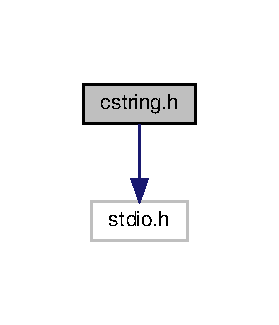
\includegraphics[width=134pt]{cstring_8h__incl}
\end{center}
\end{figure}
\subsection*{Macros}
\begin{DoxyCompactItemize}
\item 
\mbox{\Hypertarget{cstring_8h_aa93f0eb578d23995850d61f7d61c55c1}\label{cstring_8h_aa93f0eb578d23995850d61f7d61c55c1}} 
\#define {\bfseries F\+A\+L\+SE}~0
\item 
\mbox{\Hypertarget{cstring_8h_aa8cecfc5c5c054d2875c03e77b7be15d}\label{cstring_8h_aa8cecfc5c5c054d2875c03e77b7be15d}} 
\#define {\bfseries T\+R\+UE}~1
\item 
\mbox{\Hypertarget{cstring_8h_a1ca888bd091694c05472e1b91df1a97b}\label{cstring_8h_a1ca888bd091694c05472e1b91df1a97b}} 
\#define {\bfseries D\+L\+L\+\_\+\+E\+X\+P\+O\+RT}
\end{DoxyCompactItemize}
\subsection*{Typedefs}
\begin{DoxyCompactItemize}
\item 
\mbox{\Hypertarget{cstring_8h_af492d2bddcb2befacb3aa03dcdf9aafd}\label{cstring_8h_af492d2bddcb2befacb3aa03dcdf9aafd}} 
typedef char {\bfseries B\+O\+OL}
\end{DoxyCompactItemize}
\subsection*{Functions}
\begin{DoxyCompactItemize}
\item 
D\+L\+L\+\_\+\+E\+X\+P\+O\+RT \hyperlink{boolean_8h_a3e5b8192e7d9ffaf3542f1210aec18dd}{B\+O\+OL} \hyperlink{cstring_8h_a788b79461659ad8e79a9164af28d8ef2}{string\+\_\+is\+\_\+equal} (const char $\ast$a, const char $\ast$b)
\begin{DoxyCompactList}\small\item\em Check whether two strings are equal. \end{DoxyCompactList}\item 
D\+L\+L\+\_\+\+E\+X\+P\+O\+RT \hyperlink{boolean_8h_a3e5b8192e7d9ffaf3542f1210aec18dd}{B\+O\+OL} \hyperlink{cstring_8h_ad17149d107c4366f280da504df45cc10}{string\+\_\+starts\+\_\+with} (const char $\ast$a, const char $\ast$b)
\begin{DoxyCompactList}\small\item\em Check whether string {\itshape a} starts with string {\itshape b}. \end{DoxyCompactList}\item 
D\+L\+L\+\_\+\+E\+X\+P\+O\+RT \hyperlink{boolean_8h_a3e5b8192e7d9ffaf3542f1210aec18dd}{B\+O\+OL} \hyperlink{cstring_8h_ae0bb75ef00bf73fe720b76c56c98325f}{string\+\_\+contains} (const char $\ast$a, const char $\ast$b)
\begin{DoxyCompactList}\small\item\em Check whether string {\itshape a} contains string {\itshape b}. \end{DoxyCompactList}\item 
D\+L\+L\+\_\+\+E\+X\+P\+O\+RT \hyperlink{boolean_8h_a3e5b8192e7d9ffaf3542f1210aec18dd}{B\+O\+OL} \hyperlink{cstring_8h_a4b78c493fbd5c995fd8b1edc5067caf2}{string\+\_\+is\+\_\+space\+\_\+only} (const char $\ast$s)
\begin{DoxyCompactList}\small\item\em Check whether string {\itshape s} composes of only spaces. \end{DoxyCompactList}\item 
D\+L\+L\+\_\+\+E\+X\+P\+O\+RT char $\ast$ \hyperlink{cstring_8h_a5594f2b0ce2c840820c0a28fc44b7956}{string\+\_\+allocate} (const char $\ast$s)
\begin{DoxyCompactList}\small\item\em Allocate a new string out of string {\itshape s}. \end{DoxyCompactList}\item 
D\+L\+L\+\_\+\+E\+X\+P\+O\+RT char $\ast$ \hyperlink{cstring_8h_a4f33944441c46a997af3ebd1eeed1e82}{string\+\_\+allocate\+\_\+substring} (const char $\ast$s, size\+\_\+t from, size\+\_\+t to)
\begin{DoxyCompactList}\small\item\em Allocate a new substring out of string {\itshape s} from {\itshape from} to {\itshape to}. \end{DoxyCompactList}\item 
D\+L\+L\+\_\+\+E\+X\+P\+O\+RT F\+I\+LE $\ast$ \hyperlink{cstring_8h_a28b2afbc73cc0806bbec57eb1da1d6ec}{string\+\_\+to\+\_\+stream} (char $\ast$s)
\begin{DoxyCompactList}\small\item\em Convert a string to a file stream. \end{DoxyCompactList}\end{DoxyCompactItemize}


\subsection{Detailed Description}
Utility functions for C strings. 

\begin{DoxyAuthor}{Author}
Michael Chen 
\end{DoxyAuthor}
\begin{DoxyCopyright}{Copyright}
M\+IT
\end{DoxyCopyright}
{\bfseries \hyperlink{cstring_8h}{cstring.\+h}} and {\bfseries cstring.\+c} only support null-\/terminated {\ttfamily char} array. 

\subsection{Function Documentation}
\mbox{\Hypertarget{cstring_8h_a5594f2b0ce2c840820c0a28fc44b7956}\label{cstring_8h_a5594f2b0ce2c840820c0a28fc44b7956}} 
\index{cstring.\+h@{cstring.\+h}!string\+\_\+allocate@{string\+\_\+allocate}}
\index{string\+\_\+allocate@{string\+\_\+allocate}!cstring.\+h@{cstring.\+h}}
\subsubsection{\texorpdfstring{string\+\_\+allocate()}{string\_allocate()}}
{\footnotesize\ttfamily D\+L\+L\+\_\+\+E\+X\+P\+O\+RT char$\ast$ string\+\_\+allocate (\begin{DoxyParamCaption}\item[{const char $\ast$}]{s }\end{DoxyParamCaption})}



Allocate a new string out of string {\itshape s}. 


\begin{DoxyParams}{Parameters}
{\em s} & The source string. \\
\hline
\end{DoxyParams}
\begin{DoxyReturn}{Returns}
char $\ast$ 
\end{DoxyReturn}
\begin{DoxyWarning}{Warning}
Free the memory of the returning string by yourself. 
\end{DoxyWarning}
\mbox{\Hypertarget{cstring_8h_a4f33944441c46a997af3ebd1eeed1e82}\label{cstring_8h_a4f33944441c46a997af3ebd1eeed1e82}} 
\index{cstring.\+h@{cstring.\+h}!string\+\_\+allocate\+\_\+substring@{string\+\_\+allocate\+\_\+substring}}
\index{string\+\_\+allocate\+\_\+substring@{string\+\_\+allocate\+\_\+substring}!cstring.\+h@{cstring.\+h}}
\subsubsection{\texorpdfstring{string\+\_\+allocate\+\_\+substring()}{string\_allocate\_substring()}}
{\footnotesize\ttfamily D\+L\+L\+\_\+\+E\+X\+P\+O\+RT char$\ast$ string\+\_\+allocate\+\_\+substring (\begin{DoxyParamCaption}\item[{const char $\ast$}]{s,  }\item[{size\+\_\+t}]{from,  }\item[{size\+\_\+t}]{to }\end{DoxyParamCaption})}



Allocate a new substring out of string {\itshape s} from {\itshape from} to {\itshape to}. 


\begin{DoxyParams}{Parameters}
{\em s} & The source string. \\
\hline
{\em from} & The start index of the substring. \\
\hline
{\em to} & The end index of the substring \\
\hline
\end{DoxyParams}
\begin{DoxyReturn}{Returns}
char $\ast$ 
\end{DoxyReturn}
\begin{DoxyWarning}{Warning}
Free the memory of the returning string by yourself. 
\end{DoxyWarning}
\mbox{\Hypertarget{cstring_8h_ae0bb75ef00bf73fe720b76c56c98325f}\label{cstring_8h_ae0bb75ef00bf73fe720b76c56c98325f}} 
\index{cstring.\+h@{cstring.\+h}!string\+\_\+contains@{string\+\_\+contains}}
\index{string\+\_\+contains@{string\+\_\+contains}!cstring.\+h@{cstring.\+h}}
\subsubsection{\texorpdfstring{string\+\_\+contains()}{string\_contains()}}
{\footnotesize\ttfamily D\+L\+L\+\_\+\+E\+X\+P\+O\+RT \hyperlink{boolean_8h_a3e5b8192e7d9ffaf3542f1210aec18dd}{B\+O\+OL} string\+\_\+contains (\begin{DoxyParamCaption}\item[{const char $\ast$}]{a,  }\item[{const char $\ast$}]{b }\end{DoxyParamCaption})}



Check whether string {\itshape a} contains string {\itshape b}. 


\begin{DoxyParams}{Parameters}
{\em a} & The source string. \\
\hline
{\em b} & The target string. \\
\hline
\end{DoxyParams}
\begin{DoxyReturn}{Returns}
B\+O\+OL 
\end{DoxyReturn}
\mbox{\Hypertarget{cstring_8h_a788b79461659ad8e79a9164af28d8ef2}\label{cstring_8h_a788b79461659ad8e79a9164af28d8ef2}} 
\index{cstring.\+h@{cstring.\+h}!string\+\_\+is\+\_\+equal@{string\+\_\+is\+\_\+equal}}
\index{string\+\_\+is\+\_\+equal@{string\+\_\+is\+\_\+equal}!cstring.\+h@{cstring.\+h}}
\subsubsection{\texorpdfstring{string\+\_\+is\+\_\+equal()}{string\_is\_equal()}}
{\footnotesize\ttfamily D\+L\+L\+\_\+\+E\+X\+P\+O\+RT \hyperlink{boolean_8h_a3e5b8192e7d9ffaf3542f1210aec18dd}{B\+O\+OL} string\+\_\+is\+\_\+equal (\begin{DoxyParamCaption}\item[{const char $\ast$}]{a,  }\item[{const char $\ast$}]{b }\end{DoxyParamCaption})}



Check whether two strings are equal. 


\begin{DoxyParams}{Parameters}
{\em a} & The first string. \\
\hline
{\em b} & The second string. \\
\hline
\end{DoxyParams}
\begin{DoxyReturn}{Returns}
B\+O\+OL 
\end{DoxyReturn}
\mbox{\Hypertarget{cstring_8h_a4b78c493fbd5c995fd8b1edc5067caf2}\label{cstring_8h_a4b78c493fbd5c995fd8b1edc5067caf2}} 
\index{cstring.\+h@{cstring.\+h}!string\+\_\+is\+\_\+space\+\_\+only@{string\+\_\+is\+\_\+space\+\_\+only}}
\index{string\+\_\+is\+\_\+space\+\_\+only@{string\+\_\+is\+\_\+space\+\_\+only}!cstring.\+h@{cstring.\+h}}
\subsubsection{\texorpdfstring{string\+\_\+is\+\_\+space\+\_\+only()}{string\_is\_space\_only()}}
{\footnotesize\ttfamily D\+L\+L\+\_\+\+E\+X\+P\+O\+RT \hyperlink{boolean_8h_a3e5b8192e7d9ffaf3542f1210aec18dd}{B\+O\+OL} string\+\_\+is\+\_\+space\+\_\+only (\begin{DoxyParamCaption}\item[{const char $\ast$}]{s }\end{DoxyParamCaption})}



Check whether string {\itshape s} composes of only spaces. 


\begin{DoxyParams}{Parameters}
{\em s} & The source string. \\
\hline
\end{DoxyParams}
\begin{DoxyReturn}{Returns}
B\+O\+OL
\end{DoxyReturn}
string\+\_\+is\+\_\+space\+\_\+only will always skip end of line. \mbox{\Hypertarget{cstring_8h_ad17149d107c4366f280da504df45cc10}\label{cstring_8h_ad17149d107c4366f280da504df45cc10}} 
\index{cstring.\+h@{cstring.\+h}!string\+\_\+starts\+\_\+with@{string\+\_\+starts\+\_\+with}}
\index{string\+\_\+starts\+\_\+with@{string\+\_\+starts\+\_\+with}!cstring.\+h@{cstring.\+h}}
\subsubsection{\texorpdfstring{string\+\_\+starts\+\_\+with()}{string\_starts\_with()}}
{\footnotesize\ttfamily D\+L\+L\+\_\+\+E\+X\+P\+O\+RT \hyperlink{boolean_8h_a3e5b8192e7d9ffaf3542f1210aec18dd}{B\+O\+OL} string\+\_\+starts\+\_\+with (\begin{DoxyParamCaption}\item[{const char $\ast$}]{a,  }\item[{const char $\ast$}]{b }\end{DoxyParamCaption})}



Check whether string {\itshape a} starts with string {\itshape b}. 


\begin{DoxyParams}{Parameters}
{\em a} & The source string. \\
\hline
{\em b} & The target string. \\
\hline
\end{DoxyParams}
\begin{DoxyReturn}{Returns}
B\+O\+OL 
\end{DoxyReturn}
\mbox{\Hypertarget{cstring_8h_a28b2afbc73cc0806bbec57eb1da1d6ec}\label{cstring_8h_a28b2afbc73cc0806bbec57eb1da1d6ec}} 
\index{cstring.\+h@{cstring.\+h}!string\+\_\+to\+\_\+stream@{string\+\_\+to\+\_\+stream}}
\index{string\+\_\+to\+\_\+stream@{string\+\_\+to\+\_\+stream}!cstring.\+h@{cstring.\+h}}
\subsubsection{\texorpdfstring{string\+\_\+to\+\_\+stream()}{string\_to\_stream()}}
{\footnotesize\ttfamily D\+L\+L\+\_\+\+E\+X\+P\+O\+RT F\+I\+LE$\ast$ string\+\_\+to\+\_\+stream (\begin{DoxyParamCaption}\item[{char $\ast$}]{s }\end{DoxyParamCaption})}



Convert a string to a file stream. 


\begin{DoxyParams}{Parameters}
{\em s} & The source string. \\
\hline
\end{DoxyParams}
\begin{DoxyReturn}{Returns}
F\+I\+LE $\ast$ 
\end{DoxyReturn}
\begin{DoxyWarning}{Warning}
Close the file stream by yourself.
\end{DoxyWarning}
Internally, the returning file stream is a temporary file. 
\hypertarget{platform_8h}{}\section{platform.\+h File Reference}
\label{platform_8h}\index{platform.\+h@{platform.\+h}}


Platform-\/specific data.  


\subsection*{Macros}
\begin{DoxyCompactItemize}
\item 
\#define \hyperlink{platform_8h_aa3d2b101ea5e31185ae18e499d30ed11}{E\+N\+D\+\_\+\+O\+F\+\_\+\+L\+I\+NE}~\char`\"{}\textbackslash{}n\char`\"{}
\begin{DoxyCompactList}\small\item\em End of line of specific host. \end{DoxyCompactList}\item 
\#define \hyperlink{platform_8h_af1e88bb4b1ff9546e6803eec85e0684c}{D\+I\+R\+E\+C\+T\+O\+R\+Y\+\_\+\+S\+E\+P\+A\+R\+A\+T\+OR}~\char`\"{}/\char`\"{}
\begin{DoxyCompactList}\small\item\em Directory separator of specific host. \end{DoxyCompactList}\item 
\#define \hyperlink{platform_8h_a532211c2f305b447fcfaf4b746756699}{S\+E\+A\+R\+C\+H\+\_\+\+P\+A\+T\+H\+\_\+\+S\+E\+P\+A\+R\+A\+T\+OR}~\char`\"{}\+:\char`\"{}
\begin{DoxyCompactList}\small\item\em Search path separator of specific host. \end{DoxyCompactList}\end{DoxyCompactItemize}


\subsection{Detailed Description}
Platform-\/specific data. 

\begin{DoxyAuthor}{Author}
Michelle Chen 
\end{DoxyAuthor}
\begin{DoxyCopyright}{Copyright}
M\+IT
\end{DoxyCopyright}
The macro definitions seen in this document represent the platform data of Unix. 

\subsection{Macro Definition Documentation}
\mbox{\Hypertarget{platform_8h_af1e88bb4b1ff9546e6803eec85e0684c}\label{platform_8h_af1e88bb4b1ff9546e6803eec85e0684c}} 
\index{platform.\+h@{platform.\+h}!D\+I\+R\+E\+C\+T\+O\+R\+Y\+\_\+\+S\+E\+P\+A\+R\+A\+T\+OR@{D\+I\+R\+E\+C\+T\+O\+R\+Y\+\_\+\+S\+E\+P\+A\+R\+A\+T\+OR}}
\index{D\+I\+R\+E\+C\+T\+O\+R\+Y\+\_\+\+S\+E\+P\+A\+R\+A\+T\+OR@{D\+I\+R\+E\+C\+T\+O\+R\+Y\+\_\+\+S\+E\+P\+A\+R\+A\+T\+OR}!platform.\+h@{platform.\+h}}
\subsubsection{\texorpdfstring{D\+I\+R\+E\+C\+T\+O\+R\+Y\+\_\+\+S\+E\+P\+A\+R\+A\+T\+OR}{DIRECTORY\_SEPARATOR}}
{\footnotesize\ttfamily \#define D\+I\+R\+E\+C\+T\+O\+R\+Y\+\_\+\+S\+E\+P\+A\+R\+A\+T\+OR~\char`\"{}/\char`\"{}}



Directory separator of specific host. 

Currently, D\+I\+R\+E\+C\+T\+O\+R\+Y\+\_\+\+S\+E\+P\+A\+R\+A\+T\+OR works on Windows and Unix. \mbox{\Hypertarget{platform_8h_aa3d2b101ea5e31185ae18e499d30ed11}\label{platform_8h_aa3d2b101ea5e31185ae18e499d30ed11}} 
\index{platform.\+h@{platform.\+h}!E\+N\+D\+\_\+\+O\+F\+\_\+\+L\+I\+NE@{E\+N\+D\+\_\+\+O\+F\+\_\+\+L\+I\+NE}}
\index{E\+N\+D\+\_\+\+O\+F\+\_\+\+L\+I\+NE@{E\+N\+D\+\_\+\+O\+F\+\_\+\+L\+I\+NE}!platform.\+h@{platform.\+h}}
\subsubsection{\texorpdfstring{E\+N\+D\+\_\+\+O\+F\+\_\+\+L\+I\+NE}{END\_OF\_LINE}}
{\footnotesize\ttfamily \#define E\+N\+D\+\_\+\+O\+F\+\_\+\+L\+I\+NE~\char`\"{}\textbackslash{}n\char`\"{}}



End of line of specific host. 

C will handle platform-\/specific end of line automatically. Hence, we always set E\+N\+D\+\_\+\+O\+F\+\_\+\+L\+I\+NE the same value. \mbox{\Hypertarget{platform_8h_a532211c2f305b447fcfaf4b746756699}\label{platform_8h_a532211c2f305b447fcfaf4b746756699}} 
\index{platform.\+h@{platform.\+h}!S\+E\+A\+R\+C\+H\+\_\+\+P\+A\+T\+H\+\_\+\+S\+E\+P\+A\+R\+A\+T\+OR@{S\+E\+A\+R\+C\+H\+\_\+\+P\+A\+T\+H\+\_\+\+S\+E\+P\+A\+R\+A\+T\+OR}}
\index{S\+E\+A\+R\+C\+H\+\_\+\+P\+A\+T\+H\+\_\+\+S\+E\+P\+A\+R\+A\+T\+OR@{S\+E\+A\+R\+C\+H\+\_\+\+P\+A\+T\+H\+\_\+\+S\+E\+P\+A\+R\+A\+T\+OR}!platform.\+h@{platform.\+h}}
\subsubsection{\texorpdfstring{S\+E\+A\+R\+C\+H\+\_\+\+P\+A\+T\+H\+\_\+\+S\+E\+P\+A\+R\+A\+T\+OR}{SEARCH\_PATH\_SEPARATOR}}
{\footnotesize\ttfamily \#define S\+E\+A\+R\+C\+H\+\_\+\+P\+A\+T\+H\+\_\+\+S\+E\+P\+A\+R\+A\+T\+OR~\char`\"{}\+:\char`\"{}}



Search path separator of specific host. 

Currently, S\+E\+A\+R\+C\+H\+\_\+\+P\+A\+T\+H\+\_\+\+S\+E\+P\+A\+R\+A\+T\+OR works on Windows and Unix. 
\hypertarget{print_8h}{}\section{print.\+h File Reference}
\label{print_8h}\index{print.\+h@{print.\+h}}


Console printing related macros.  


{\ttfamily \#include $<$stdio.\+h$>$}\newline
Include dependency graph for print.\+h\+:\nopagebreak
\begin{figure}[H]
\begin{center}
\leavevmode
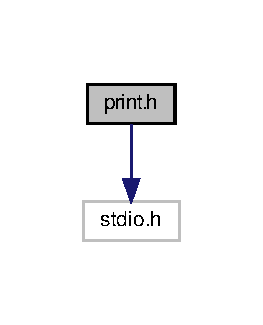
\includegraphics[width=125pt]{print_8h__incl}
\end{center}
\end{figure}
\subsection*{Macros}
\begin{DoxyCompactItemize}
\item 
\mbox{\Hypertarget{print_8h_aa3d2b101ea5e31185ae18e499d30ed11}\label{print_8h_aa3d2b101ea5e31185ae18e499d30ed11}} 
\#define {\bfseries E\+N\+D\+\_\+\+O\+F\+\_\+\+L\+I\+NE}~\char`\"{}\textbackslash{}n\char`\"{}
\item 
\#define \hyperlink{print_8h_af990e936c83edcff058ae8ec5864adec}{P\+R\+I\+NT}(format, ...)
\begin{DoxyCompactList}\small\item\em Print formated string to {\bfseries stdout} without trailing E\+OL. \end{DoxyCompactList}\item 
\#define \hyperlink{print_8h_a36f6a6453e7533808c32a37f455068a0}{P\+E\+R\+R\+OR}(format, ...)
\begin{DoxyCompactList}\small\item\em Print formated string to {\bfseries stderr} without trailing E\+OL. \end{DoxyCompactList}\item 
\#define \hyperlink{print_8h_ad5ec9098821844c0c27cd849fc930c90}{P\+U\+TS}(format, ...)
\begin{DoxyCompactList}\small\item\em Print formated string to {\bfseries stdout} with trailing E\+OL. \end{DoxyCompactList}\item 
\#define \hyperlink{print_8h_a84559fc324a4622242ee818f9025141f}{P\+U\+T\+E\+RR}(format, ...)
\begin{DoxyCompactList}\small\item\em Print formated string to {\bfseries stderr} with trailing E\+OL. \end{DoxyCompactList}\item 
\#define \hyperlink{print_8h_a994994514490b70ee6a5dd679f28acbc}{D\+E\+B\+U\+G\+\_\+\+I\+N\+FO}(format, ...)
\begin{DoxyCompactList}\small\item\em Print formated debug message to {\bfseries stderr} with trailing E\+OL. \end{DoxyCompactList}\end{DoxyCompactItemize}


\subsection{Detailed Description}
Console printing related macros. 

\begin{DoxyAuthor}{Author}
Michael Chen 
\end{DoxyAuthor}
\begin{DoxyCopyright}{Copyright}
M\+IT
\end{DoxyCopyright}
The macro definition seen in this document represent the platform data of Unix. 

\subsection{Macro Definition Documentation}
\mbox{\Hypertarget{print_8h_a994994514490b70ee6a5dd679f28acbc}\label{print_8h_a994994514490b70ee6a5dd679f28acbc}} 
\index{print.\+h@{print.\+h}!D\+E\+B\+U\+G\+\_\+\+I\+N\+FO@{D\+E\+B\+U\+G\+\_\+\+I\+N\+FO}}
\index{D\+E\+B\+U\+G\+\_\+\+I\+N\+FO@{D\+E\+B\+U\+G\+\_\+\+I\+N\+FO}!print.\+h@{print.\+h}}
\subsubsection{\texorpdfstring{D\+E\+B\+U\+G\+\_\+\+I\+N\+FO}{DEBUG\_INFO}}
{\footnotesize\ttfamily \#define D\+E\+B\+U\+G\+\_\+\+I\+N\+FO(\begin{DoxyParamCaption}\item[{}]{format,  }\item[{}]{... }\end{DoxyParamCaption})}

{\bfseries Value\+:}
\begin{DoxyCode}
\{ \(\backslash\)
        fprintf(stderr, \textcolor{stringliteral}{"(%s:%d) "} format \textcolor{stringliteral}{"%s"}, \(\backslash\)
            \_\_FILE\_\_, \_\_LINE\_\_, ##\_\_VA\_ARGS\_\_, \hyperlink{platform_8h_aa3d2b101ea5e31185ae18e499d30ed11}{END\_OF\_LINE}); \(\backslash\)
    \}
\end{DoxyCode}


Print formated debug message to {\bfseries stderr} with trailing E\+OL. 

{\bfseries D\+E\+B\+U\+G\+\_\+\+I\+N\+FO} works similarly to {\bfseries P\+U\+T\+E\+RR} but adds source file and line number. Hence, developers can track the location of the message more easily. \mbox{\Hypertarget{print_8h_a36f6a6453e7533808c32a37f455068a0}\label{print_8h_a36f6a6453e7533808c32a37f455068a0}} 
\index{print.\+h@{print.\+h}!P\+E\+R\+R\+OR@{P\+E\+R\+R\+OR}}
\index{P\+E\+R\+R\+OR@{P\+E\+R\+R\+OR}!print.\+h@{print.\+h}}
\subsubsection{\texorpdfstring{P\+E\+R\+R\+OR}{PERROR}}
{\footnotesize\ttfamily \#define P\+E\+R\+R\+OR(\begin{DoxyParamCaption}\item[{}]{format,  }\item[{}]{... }\end{DoxyParamCaption})}

{\bfseries Value\+:}
\begin{DoxyCode}
\{ \(\backslash\)
        fprintf(stderr, format, ##\_\_VA\_ARGS\_\_); \(\backslash\)
    \}
\end{DoxyCode}


Print formated string to {\bfseries stderr} without trailing E\+OL. 

{\bfseries P\+E\+R\+R\+OR} works as {\bfseries P\+R\+I\+NT}, but to {\bfseries stderr}. \mbox{\Hypertarget{print_8h_af990e936c83edcff058ae8ec5864adec}\label{print_8h_af990e936c83edcff058ae8ec5864adec}} 
\index{print.\+h@{print.\+h}!P\+R\+I\+NT@{P\+R\+I\+NT}}
\index{P\+R\+I\+NT@{P\+R\+I\+NT}!print.\+h@{print.\+h}}
\subsubsection{\texorpdfstring{P\+R\+I\+NT}{PRINT}}
{\footnotesize\ttfamily \#define P\+R\+I\+NT(\begin{DoxyParamCaption}\item[{}]{format,  }\item[{}]{... }\end{DoxyParamCaption})}

{\bfseries Value\+:}
\begin{DoxyCode}
\{ \(\backslash\)
        fprintf(stdout, format, ##\_\_VA\_ARGS\_\_); \(\backslash\)
    \}
\end{DoxyCode}


Print formated string to {\bfseries stdout} without trailing E\+OL. 

Basically, {\bfseries P\+R\+I\+NT} is just a repackaged {\itshape printf} function seen {\bfseries stdio.\+h}. \mbox{\Hypertarget{print_8h_a84559fc324a4622242ee818f9025141f}\label{print_8h_a84559fc324a4622242ee818f9025141f}} 
\index{print.\+h@{print.\+h}!P\+U\+T\+E\+RR@{P\+U\+T\+E\+RR}}
\index{P\+U\+T\+E\+RR@{P\+U\+T\+E\+RR}!print.\+h@{print.\+h}}
\subsubsection{\texorpdfstring{P\+U\+T\+E\+RR}{PUTERR}}
{\footnotesize\ttfamily \#define P\+U\+T\+E\+RR(\begin{DoxyParamCaption}\item[{}]{format,  }\item[{}]{... }\end{DoxyParamCaption})}

{\bfseries Value\+:}
\begin{DoxyCode}
\{ \(\backslash\)
        fprintf(stderr, format \textcolor{stringliteral}{"%s"}, ##\_\_VA\_ARGS\_\_, \hyperlink{platform_8h_aa3d2b101ea5e31185ae18e499d30ed11}{END\_OF\_LINE}); \(\backslash\)
    \}
\end{DoxyCode}


Print formated string to {\bfseries stderr} with trailing E\+OL. 

The E\+OL will change according to the host environment. \mbox{\Hypertarget{print_8h_ad5ec9098821844c0c27cd849fc930c90}\label{print_8h_ad5ec9098821844c0c27cd849fc930c90}} 
\index{print.\+h@{print.\+h}!P\+U\+TS@{P\+U\+TS}}
\index{P\+U\+TS@{P\+U\+TS}!print.\+h@{print.\+h}}
\subsubsection{\texorpdfstring{P\+U\+TS}{PUTS}}
{\footnotesize\ttfamily \#define P\+U\+TS(\begin{DoxyParamCaption}\item[{}]{format,  }\item[{}]{... }\end{DoxyParamCaption})}

{\bfseries Value\+:}
\begin{DoxyCode}
\{ \(\backslash\)
        fprintf(stdout, format \textcolor{stringliteral}{"%s"}, ##\_\_VA\_ARGS\_\_, \hyperlink{platform_8h_aa3d2b101ea5e31185ae18e499d30ed11}{END\_OF\_LINE}); \(\backslash\)
    \}
\end{DoxyCode}


Print formated string to {\bfseries stdout} with trailing E\+OL. 

The E\+OL will change according to the host environment. 
%--- End generated contents ---

% Index
\backmatter
\newpage
\phantomsection
\clearemptydoublepage
\addcontentsline{toc}{chapter}{Index}
\printindex

\end{document}
